\chapter{Introduction}

%%%%%%%%%%%%%%%%%%%%%%%%%%%%%%%%%%%%%%%%%%%%%%%%%%%%%%%%%%%%%%%%%%%%%%%%%%%%%%%%%%%%%%%%%%%%%%%%%%%

\section{Disclaimer}

This reference describes syntax and semantics of the nML architecture
description language. It covers only language facilities supported by the ISP RAS
version of nML. It may differ from documentation provided by other vendors as
there are differences in language implementations.

%%%%%%%%%%%%%%%%%%%%%%%%%%%%%%%%%%%%%%%%%%%%%%%%%%%%%%%%%%%%%%%%%%%%%%%%%%%%%%%%%%%%%%%%%%%%%%%%%%%

\section{Overview}

nML is an architecture description language (ADL) used to describe the
instruction set architecture (ISA) of an arbitrary microprocessor. It is a
flexible and easy-to-use language based on attribute grammar. nML was designed
to provide a retargetable way to specify microprocessor architecture for
various microprocessor-related software tools including instruction-set
simulators, assemblers, disassemblers, compiler back-ends etc. It works at
the instruction-set level concentrating on behavioral properties and hiding
implementation details. An nML specification represents a programmer's model
of the microprocessor which covers the following aspects:

\begin{itemize}
\item supported data types;
\item registers and memory;
\item addressing modes;
\item syntax and semantics of instructions.
\end{itemize}

nML uses a hierarchical tree-like structure to describe an instruction set.
Such a structure facilitates grouping related instructions and sharing their
common parts. An instruction is described as a path in the tree from the root
node to a leaf node. The set of all possible paths represents an instruction
set. A node describes a primitive operation responsible for some task within
an instruction. Each node has certain attributes that can be shared with its
descendants. Actions performed by instructions are described as operations
with registers and memory represented by bit vectors of arbitrary size.

A specification in nML starts with definitions of types and global constants.
For example, a type definition for a 32-bit unsigned integer looks as follows:

\begin{lstlisting}[language=C]
let WORD_SIZE = 32
type WORD = card(WORD_SIZE)
\end{lstlisting}

Type definitions and constants can be used to describe registers and memory.
In addition to registers and memory, it is also possible to define temporary
variables that are internal abstractions provided by nML to store intermediate
results of operations. They do not correspond to any data storage in real
hardware and do not save their data across instruction calls. Also, there is
often a need to specify some properties of the described model. For this
purpose, special constants are used. For example, the code below defines
general-purpose registers, memory and a temporary variable. Also, it includes
a special constant to establish a correspondence between the general purpose
register number 15 and the program counter (PC). Here is the code:

\begin{lstlisting}
reg GPR[32, WORD]
mem M[2 ** 20, BYTE]
var carry[1, BIT]
let PC = "GPR[15]"
\end{lstlisting}

As stated above, an instruction set is described as a tree of primitive
operations. There two kinds of primitives: operations and addressing modes.
Operations describe parts of instructions responsible for specific tasks and
can be used as leaf and root nodes. Addressing modes are aimed to customize
operations (for example, they encapsulate rules for accessing microprocessor
resources). They can only be used as leaf nodes. For example, here are
simplified examples of operation and addressing mode specifications:

\begin{lstlisting}
mode REG(i: nibble) = R[i]
syntax = format("R%d", i)
image  = format("01%4b", i)
\end{lstlisting}

\begin{lstlisting}
op Add()
syntax = "add" 
image  = "00" 
action = { DEST = SRC1 + SRC2; }
\end{lstlisting}

Operations and addressing modes have three standard attributes: syntax, image
and action. The first two specify textual and binary syntax. The third
describes semantics of the primitive. In addition, addressing modes have
a return expression that enables them to be used as variables in various
expressions. Attributes can be used by parent primitives referring to a given
primitive to describe more complex abstractions.

Primitives are arranged into a tree using production rules. There are two kinds
of production rules: AND rules and OR rules. AND rules specify parent-child
relationships where a child primitive is described as a parameter of its
parent. Here is an example of an AND rule:

\begin{lstlisting}
op arith_inst(act: Add, op1: OPRND, op2: OPRND)
\end{lstlisting}

This is the header of the {\texttt arith{\_}inst} operation that states that the
{\texttt arith{\_}inst} operation node has three child nodes: the {\texttt act} operation and the
{\texttt op1} and {\texttt op2} addressing modes. The syntax of an operation header is similar
to a function where parameter types specify the primitives the rule refers to.
Parameter can be, in turn, parameterized with other primitives (they will be
encapsulated behind attributes). For this reason child nodes represent
independent instances that are accessed from their parent node via parameters.
OR rules specify alternatives. This means that a group of primitives is united
under some alias so that each of them can used when this alias is specified in
an AND rule. An OR rule looks as follows:

\begin{lstlisting}
op Add_Sub_Mov = Add | Sub | Mov
\end{lstlisting}

Figure 1 displays a tree path describing the {\texttt mov} instruction from an
imaginary instruction set. This instruction copies data from one register to
another. The root operation of the instruction is called {\texttt instruction}.
According to nML conventions, the root operation is always called {\texttt instruction}
and it specifies the point from which all paths describing specific
instructions start. The {\texttt instruction} operation can be defined either as AND or
OR rule. In the latter case, there are several starting points. Usually root
operations holds some common properties and perform common actions (such as
increment of the program counter). In the given example, the root operation is
linked to the {\texttt Arithm} operation with the help of an AND rule. This operation
describes a group of arithmetic operations. It is parameterized with the
{\texttt Add{\_}Mov{\_}Sub} and {\texttt OPRND} primitives. Both of them are specified as OR rules.
The first one describes arithmetic operations that can be performed by the
{\texttt Arithm} primitive while the second one specifies supported addressing modes.
Dashed lines that connect OR-rules with their child primitives specify possible
alternative paths. Instructions are identified by the terminal operation node of
the path (in this example, it is the {\texttt Mov} node). An important note is that, to
avoid ambiguity, nodes can have only one child operation.

\begin{figure}
\centering
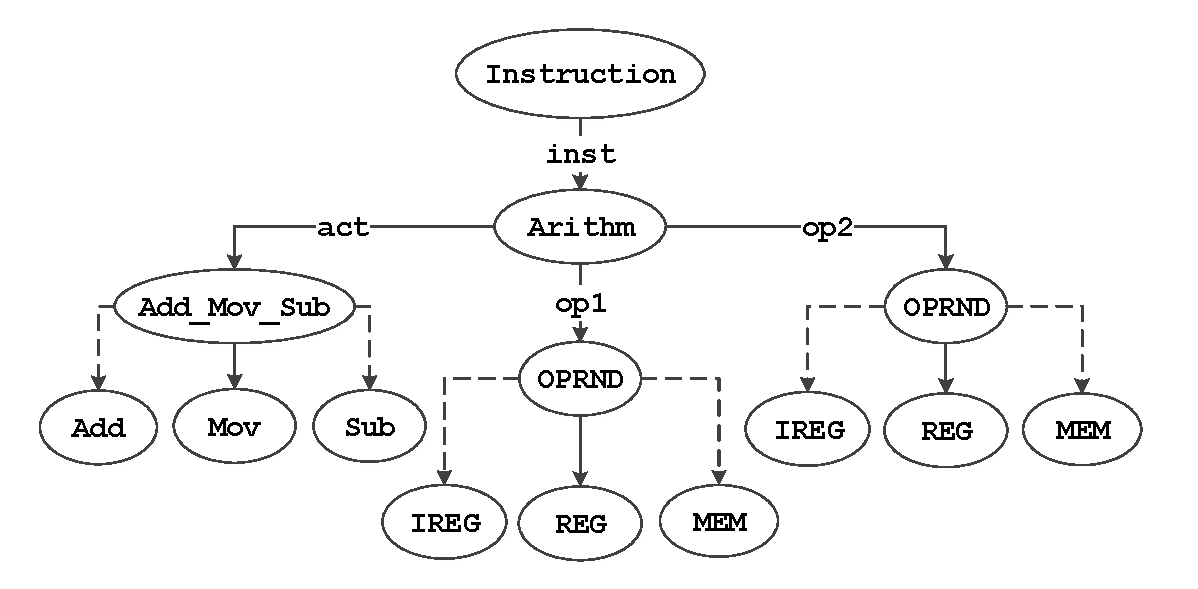
\includegraphics [width=0.85\textwidth]
{figures/figure1.pdf}
\caption{Operation tree for the Mov instruction}
\label{nml-instruction-tree}
\end{figure}

The syntax of nML resembles the syntax of the pseudocode used in microprocessor
architecture manuals to describe instruction semantics. For example, here is the
description of instruction ADD from the MIPS64 manual:

\begin{lstlisting}[mathescape=true]
if NotWordValue(GPR[rs]) or NotWordValue(GPR[rt]) then
  UNPREDICTABLE
endif
temp $\leftarrow$ GPR[rs]$_{31}$||GPR[rs]$_{31..0}$) + (GPR[rt]$_{31}$||GPR[rt]$_{31..0}$)
if temp$_{32}$ $\neq$ temp$_{31}$ then
  SignalException(IntegerOverflow)
else
  GPR[rd] $\leftarrow$ sign_extend(temp$_{31..0}$)
endif
\end{lstlisting}

Such a description can be translated to nML with minimal effort. Providing that
all needed data types, resources and operations describing common functionality
of instructions have already been specified, the specification of the ADD
instruction (or, to be more precise, the terminal operation that distinguishes
it from other similar instructions) will look as follows:

\begin{lstlisting}
op add (rd: R, rs: R, rt: R)
  syntax = format("add %s, %s, %s", rd.syntax, rs.syntax, rt.syntax)
  image  = format("000000%5s%5s%5s00000100000", rs.image, rt.image, rd.image)
  action = {
    if sign_extend(WORD, rs<31>) != rs<63..32> ||
       sign_extend(WORD, rt<31>) != rt<63..32> then
      unpredicted;
    endif;

    temp33 = rs<31>::rs<31..0> + rt<31>::rt<31..0>;
    if temp33<32> != temp33<31> then
      C0_EPC = CIA;
      exception("IntegerOverflow");
    else
      rd = sign_extend(DWORD, temp33<31..0>);
    endif;
  }
\end{lstlisting}

As we can see, describing an instruction based on an instruction set manual is
a relatively easy task that can be performed by a verification engineer who
does not have significant programming skills.
